% \includepdf[pages=-]{doc/Fichamento.pdf}%
\label{apendice:ativos}

% Este apêndice descreve detalhadamente, acompanhado de resultados gráficos, as análises realizadas para experimentos com ativos ativos individuais no \acrlong{MAR}.

\section{Alocação do Ativo PETR3}

Dentre os experimentos realizados para os ativos individuais, o primeiro a ser analisado foi o PETR3. O experimento foi realizado utilizando a mesma janela de valor $6$ encontrada nos experimentos do \acrshort{MPM}, e com R\$$10.000$ de investimento inicial. As \refFigs{ptr_clean_qval}{petr_clean_act}, demonstram todos os dados obtidos nas 200 épocas de treino e em seus testes por época. A \refFig{petr_clean_ret} apresenta o comportamento do retorno médio obtido por episódios de treino e teste. Apesar das altas oscilações apresentadas, no final da simulação o retorno médio alcança o valor de $92.21$ e $82.272$ em treino e teste respectivamente, o que demonstra uma devida conversão do aprendizado.

\figura{img/ddpg/petr3/clean/return}{PETR3 - Retorno médio}{petr_clean_ret}{width=.5\linewidth}

Observa-se também, analisando a \refFig{ptr_clean_qval} e a \refFig{petr_clean_loss} que o Q-Valor médio e as funções de perda também convergiram. O Q-Valor alcança uma média de $26.36$, variando entre $203.69$ a $-73.92$, enquanto as funções de perda assumem os valores de $62.77$ e $-26.43$ para perda Q (função de aproximação do Q-Valor) e perda $\pi$ (função de aproximação da política). Apesar dos valores não estarem muito próximos de $0$, experimentos com mais quantidades de épocas foram conduzidos e sua variação não foi significante. Tal comportamento pode ser um indicativo de que o experimento encontrou um mínimo local, necessitando assim de uma modificação na formulação de ambiente ou na função de recompensa.

\begin{figure}[htbp]
    \centering 
    \begin{minipage}[b]{0.45\linewidth}
        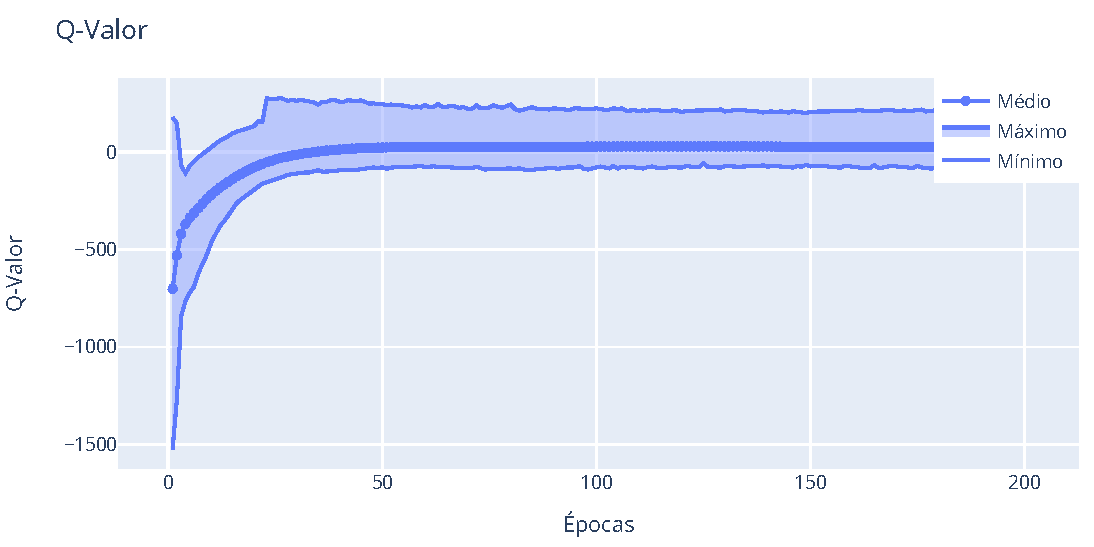
\includegraphics[width=\linewidth]{img/ddpg/petr3/clean/qval}
        \caption{PETR3 - Comportamento do QValor} 
        \label{ptr_clean_qval}
    \end{minipage}
    \quad
    \begin{minipage}[b]{0.45\linewidth}
        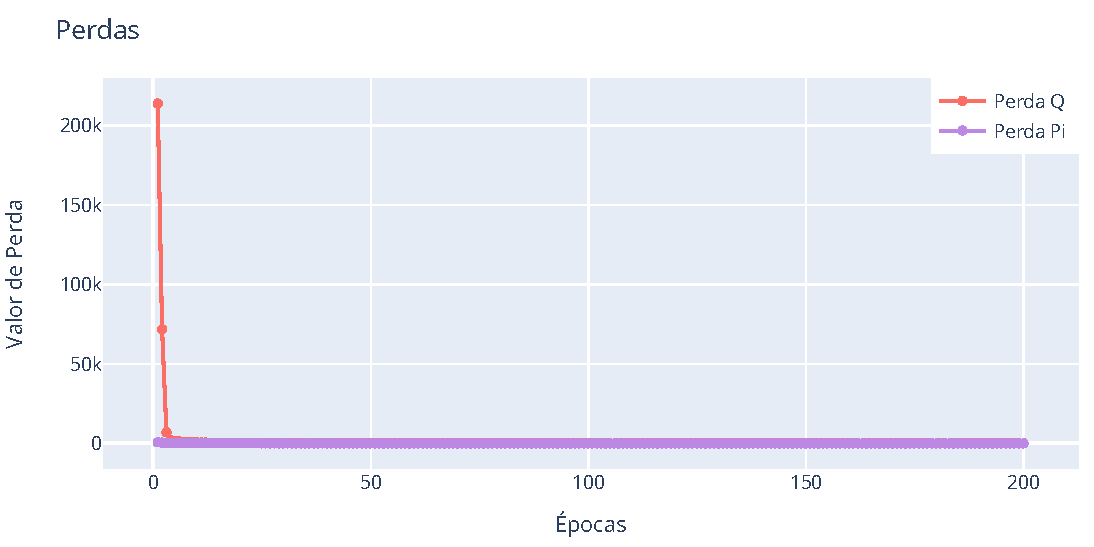
\includegraphics[width=\linewidth]{img/ddpg/petr3/clean/loss}
        \caption{PETR3 - Comportamento das funções de perda}
        \label{petr_clean_loss}
    \end{minipage}
\end{figure}

Em relação ao lucro obtido, nota-se na \refFig{petr_clean_ptrain}, que durante o treino se obteve uma alta dispersão de valores, fruto do alto ruído introduzido no treinamento, incluindo encontrar um lucro de R\$$4.670,00$ em um dos episódios. No entanto, o algoritmo não decide aproveitar o comportamento encontrado para esse lucro. 

\figura[htbp]{img/ddpg/petr3/clean/profit_train}{PETR3 - Lucro em treino}{petr_clean_ptrain}{width=.5\linewidth}

Quando o resultado do lucro é observado em teste (\refFig{petr_clean_profit}), percebe-se ainda as diversas oscilações apresentadas no treino, além de também não explorar a política com maior lucro encontrada. O fato de o algoritmo divergir de forma significativa e não explorar necessariamente o maior lucro pode estar relacionada com a formulação da função de recompensa, que não reflete exatamente o lucro obtido. No entanto, mesmo com essas variações presentes, o modelo obteve um lucro final médio em teste de R\$$1.377,00$, realizando majoritariamente ações de compra (veja a \refFig{petr_clean_act}), quase não vendendo nem esperando. Vale enfatizar que nem toda ação de compra é realizada, se o agente não possui a quantidade de dinheiro para a compra ele recebe uma punição pela ação realizada de forma incorreta, o porquê de o agente preferir uma punição a uma ação de espera é algo a ser explorado.

\begin{figure}[htbp]
    \centering 
    \begin{minipage}[b]{0.45\linewidth}
        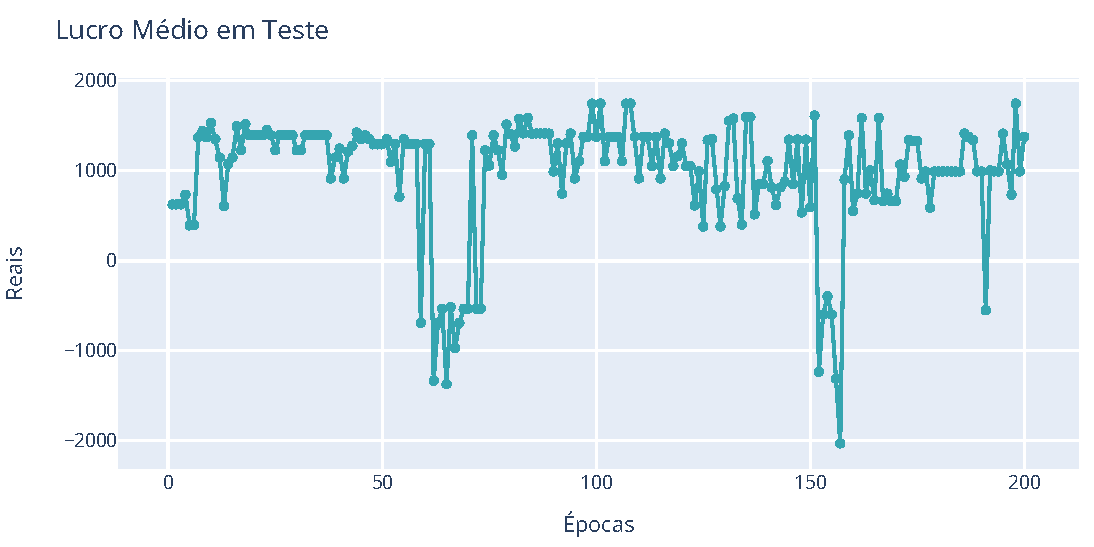
\includegraphics[width=\linewidth]{img/ddpg/petr3/clean/profit}
        \caption{PETR3 - Lucro médio em teste.} 
        \label{petr_clean_profit}
    \end{minipage}
    \quad
    \begin{minipage}[b]{0.45\linewidth}
        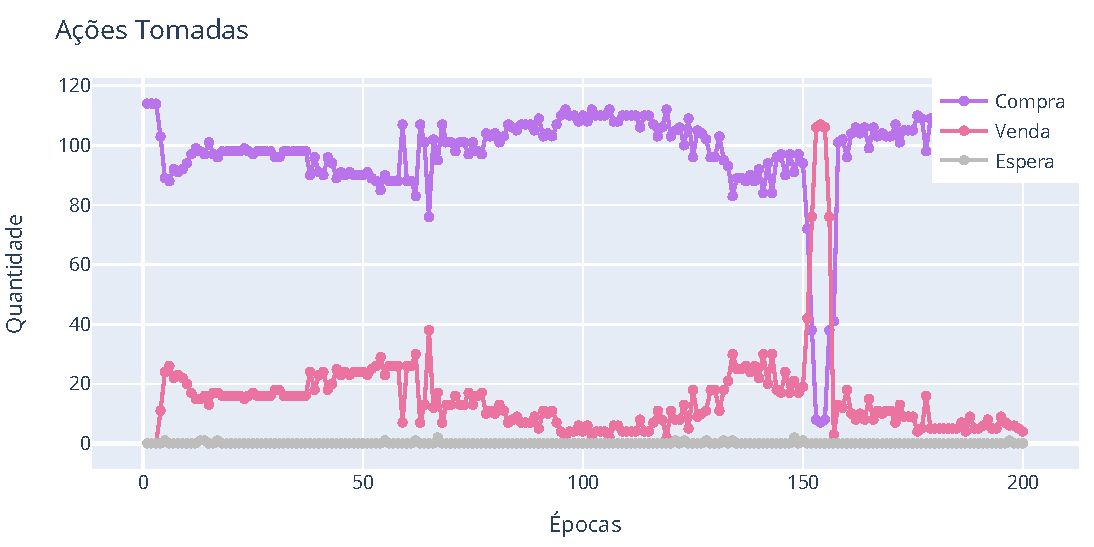
\includegraphics[width=\linewidth]{img/ddpg/petr3/clean/actions}
        \caption{PETR3 - Quantidade de ações selecionadas em teste.}
        \label{petr_clean_act}
    \end{minipage}
\end{figure}

Portanto, nota-se que o modelo, apesar de todas as adversidades encontradas, obteve um lucro de R\$$1.377,00$ no final do teste, uma rentabilidade de $13,77\%$ no total dos 6 meses. A rentabilidade encontrada é $311,04\%$ maior que da poupança e $182,75\%$ maior que o \acrshort{CDI}. No caso de um investidor seguindo uma estratégia \emph{buy and hold}, o mesmo compraria o ativo a R\$$15,01$, com $10.000$ reais esse investidor compraria $600$ cotas a R\$$9.006,00$, e sobraria $994$ reais em conta. No fim do período, as ações da PETR3 estavam valendo R\$$16,05$ e, portanto, o seu portfólio estaria valendo R\$$9.630,00$, totalizando R\$$10.624,00$ com o dinheiro em conta, uma rentabilidade de $6,24\%$ no final do período. A estratégia de investimento aprendida pelo agente para operar no ativo, possui uma rentabilidade $120,67\%$ maior que o investidor seguindo um comportamento \emph{buy and hold}.
 
\section{Alocação do Ativo VALE3}

O segundo ativo individual analisado foi o VALE3. Os experimentos realizados para este ativo possuem a mesma configuração de janela e de investimento inicial do ativo PETR3 previamente apresentado. As \refFigs{vale_clean_qval}{vale_clean_act}, demonstram todos os dados obtidos, também utilizando 200 épocas de treino e $10$ testes por época. Novamente realiza-se a análise começando pelo gráfico de retorno médio por episódios de treino e teste, demonstrados na \refFig{vale_clean_ret}. Diferentemente do ativo da PETR3, o retorno apresentado nas simulações da VALE não possui tanta oscilação, indicando uma menor exploração pelo modelo. No final da simulação, o algoritmo obtém um retorno médio de $-3.327$ para ambos treino e teste, mesmo tendo encontrado um retorno de $31,83$ ao longo de sua trajetória. 

\figura{img/ddpg/vale3/clean/return}{VALE3 - Retorno médio}{vale_clean_ret}{width=.5\linewidth}

De forma similar ao ativo anterior, analisa-se também as \refFigs{vale_clean_qval}{vale_clean_loss} para entender o comportamento do Q-Valor médio e das funções de perda. O Q-Valor obtido possui uma média de $-11.31$, variando entre $51.44$ e $-135.28$. Tal valor médio negativo de Q-Valor, junto com um mínimo tão discrepante da média justificam o retorno negativo médio obtido pelo modelo. Por outro lado, as funções de perda assumem os valores mais próximos de $0$, com $21.13$ para a aproximação do Q-Valor e $11.18$ para aproximação da política, o que pode ser um indicativo de que este modelo é mais adaptável a replicações em relação ao do ativo PETR3. 

\begin{figure}[htbp]
    \centering 
    \begin{minipage}[b]{0.45\linewidth}
        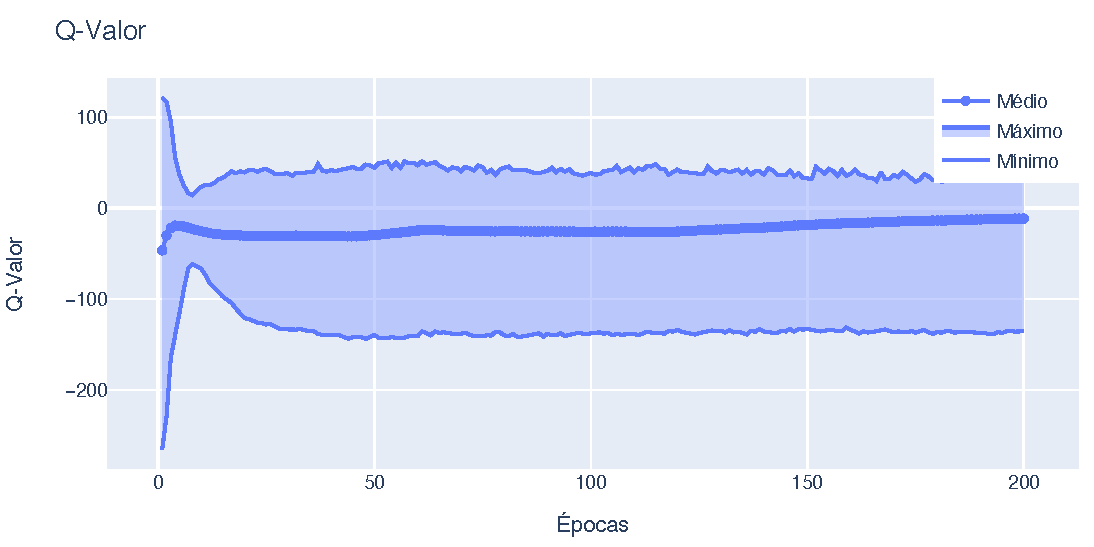
\includegraphics[width=\linewidth]{img/ddpg/vale3/clean/qval}
        \caption{VALE3 - Comportamento do QValor.} 
        \label{vale_clean_qval}
    \end{minipage}
    \quad
    \begin{minipage}[b]{0.45\linewidth}
        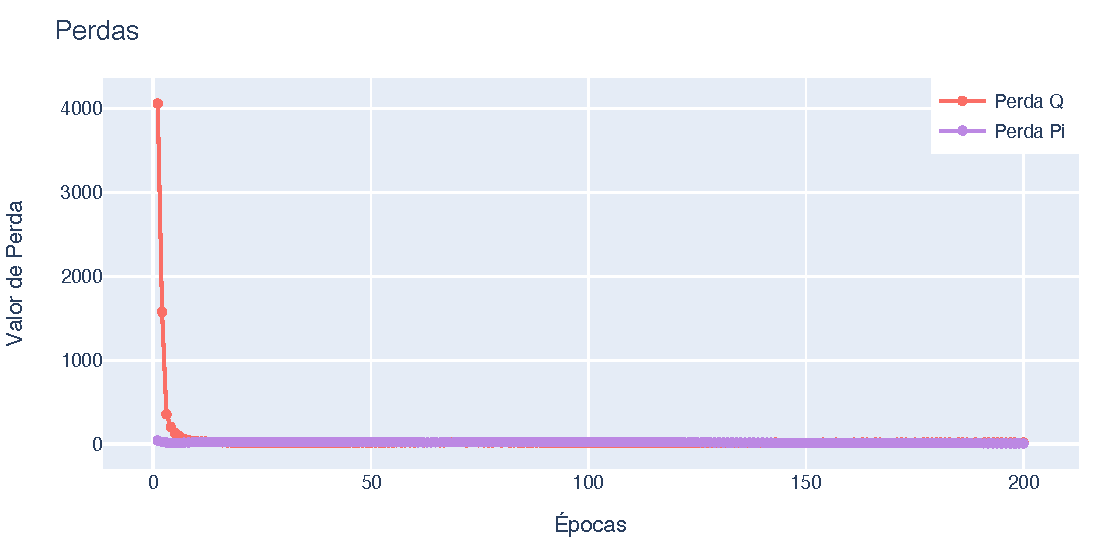
\includegraphics[width=\linewidth]{img/ddpg/vale3/clean/loss}
        \caption{VALE3 - Comportamento das funções de perda.}
        \label{vale_clean_loss}
    \end{minipage}
\end{figure}

Com base no lucro obtido durante a fase de treino, apresentado na \refFig{vale_clean_ptrain}, nota-se também uma alta dispersão dos valores chegando a encontrar lucros maiores que mil reais, mas esses não foram explorados. Observa-se que a conversão para um valor de lucro constante acontece bem mais rápida, e mesmo com o ruído presente, o treino não varia a mesma quantidade de PETR3.

\figura[htbp]{img/ddpg/vale3/clean/profit_train}{VALE3 - Lucro em treino}{vale_clean_ptrain}{width=.5\linewidth}

Quando o valor do lucro é analisado em teste (\refFig{vale_clean_profit}), percebe-se um padrão similar a média de lucro obtida no treino. O maior lucro encontrado durante a simulação foi de R\$$942,00$, no entanto, o valor final para qual o algoritmo converge é de apenas $603,00$ reais. Este comportamento reforça a hipótese de que a função de recompensa pode ser responsável pela falta de aproveitamento do agente por lucros maiores. Em relação as ações, apresentadas na \refFig{vale_clean_act}, o comportamento selecionado é discrepante com o realizado para o ativo da PETR3, realizando majoritariamente ações de venda, quase não vendendo e nunca esperando. De forma similar, enfatiza-se que nem toda ação de venda é realizada, se o agente não possui ativos para vender ele recebe uma punição pela ação realizada de forma incorreta. Também é incerto o porquê de o agente não aproveitar os comportamentos de espera.

\begin{figure}[htbp]
    \centering 
    \begin{minipage}[b]{0.45\linewidth}
        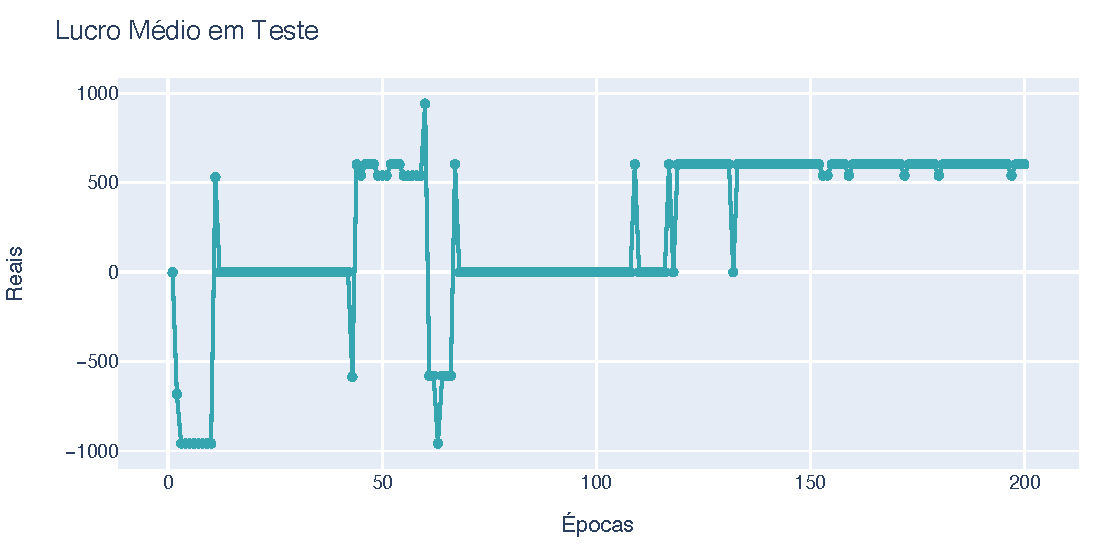
\includegraphics[width=\linewidth]{img/ddpg/vale3/clean/profit}
        \caption{VALE3 - Lucro médio em teste.} 
        \label{vale_clean_profit}
    \end{minipage}
    \quad
    \begin{minipage}[b]{0.45\linewidth}
        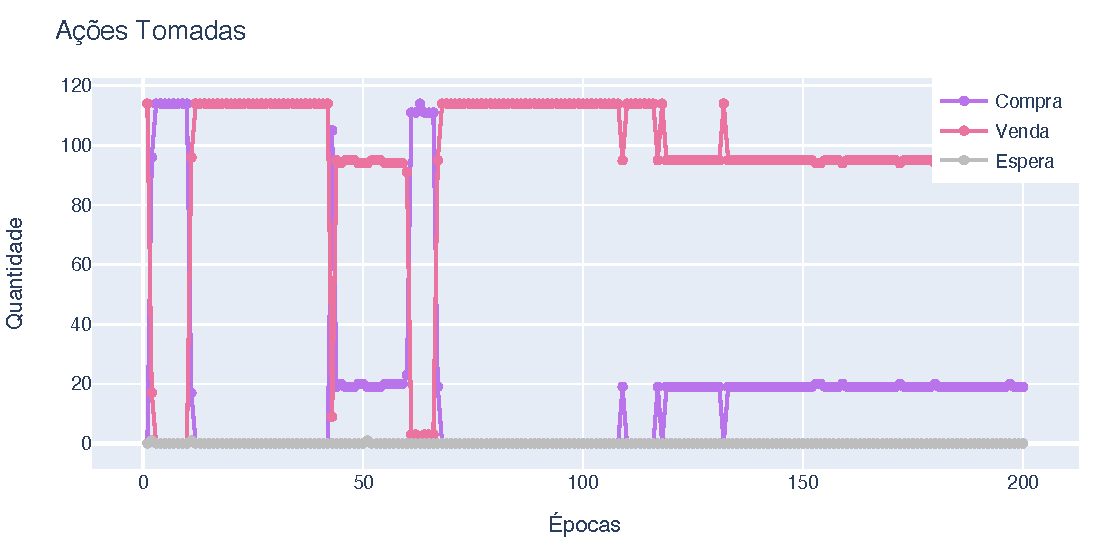
\includegraphics[width=\linewidth]{img/ddpg/vale3/clean/actions}
        \caption{VALE3 - Quantidade de ações selecionadas em teste.}
        \label{vale_clean_act}
    \end{minipage}
\end{figure}

Analisando o desempenho do modelo, percebe-se que as adversidades impactaram de forma significante a capacidade do agente lucrar, obtendo um lucro de apenas R\$$603,00$. Este lucro representa uma rentabilidade de $6,03\%$ no total dos 6 meses. No entanto, a rentabilidade, apesar de baixa, ainda oferece lucratividade $80\%$ e $23,81\%$ maior que a poupança e o CDI respectivamente. Considerando a estratégia \emph{buy and hold} de um investidor, os ativos da VALE3 seriam comprados inicialmente pelo valor de R\$$32,25$, o que permitirá a compra de $300$ cotas a R\$$9.675,00$ e sobraria R\$$325,00$ em conta. No fim do período estipulado para a simulações, as ações da VALE3 alcançariam um valor de R\$$29,06$. O investidor que tivesse alocado essa quantia nos ativos da Vale nesse período perderia $957$ reais, terminando com $8.718$ em ativos, totalizando com o saldo em carteira $9.043$, uma rentabilidade de $-9,57\%$. A estratégia de investimento aprendida pelo agente, apesar de não apresentar grandes lucros, demonstra uma aversão a perdas, sabendo parar de investir quando algum lucro foi obtido.


\section{Alocação do Ativo ABEV3}

Finalizando, o ultimo ativo individual a ser analisado foi o ABEV3. Neste ativo também foi utilizado R\$$10.000,00$ de valor inicial, mas diferentemente da PETR3 e VALE3, a janela utilizada foi de 9 dias, similar ao resultado da \acrshort{LSTM}. Os dados obtidos nos experimentos estão representados nas \refFigs{abev_clean_ret}{abev_clean_act}, onde cada experimento também acontece em $200$ épocas de treino e $10$ episódios de teste por época. A \refFig{vale_clean_ret}, apresenta o retorno médio por episódios de treino e teste. Para o ativo especifico da ABEV3, o modelo não conseguiu generalizar a ponto de obter lucros. Acredita-se que este comportamento pode ser fruto da dificuldade do agente em encontrar recompensas positivas significantes no começo da simulação, entrando em uma situação de \emph{deadlock}, onde o algoritmo da \acrshort{DDPG} falha em aprender \cite{matheron2019problem}. No final da simulação, o algoritmo obtém um retorno médio de $-61.05$ para treino e $-68.70$ para teste, mesmo tendo encontrado retornos maiores ao longo de sua trajetória. 

\figura{img/ddpg/abev3/clean/return}{ABEV3 - Retorno médio}{abev_clean_ret}{width=.5\linewidth}

A busca pelo entendimento desse comportamento para o ativo da ABEV3, segue com a análise das \refFigs{abev_clean_qval}{abev_clean_loss}. Essa análise busca entender o comportamento do Q-Valor médio e das funções de perda, que levaram a um desempenho ruim. O Q-Valor obtido possui uma média de $-27.59$, variando entre $98.05$ e $-154.09$. Em relação as funções de perda, aproximação do Q-Valor chega a $13.59$, enquanto a aproximação de $\pi$ a ultrapassa, chegando a $27.57$, claramente divergindo da política buscada.

\begin{figure}[htbp]
    \centering 
    \begin{minipage}[b]{0.45\linewidth}
        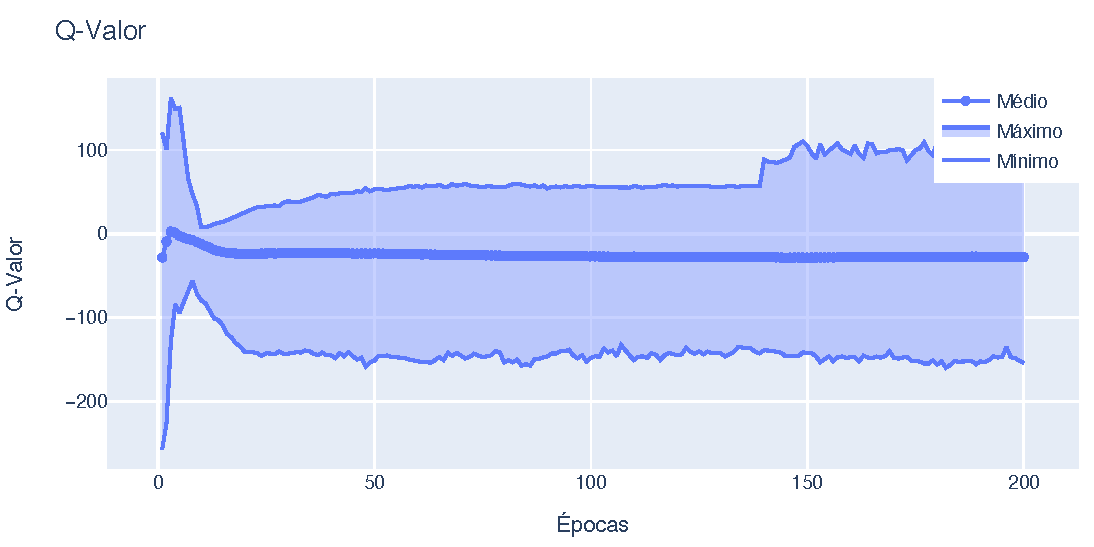
\includegraphics[width=\linewidth]{img/ddpg/abev3/clean/qval}
        \caption{ABEV3 - Comportamento do QValor.} 
        \label{abev_clean_qval}
    \end{minipage}
    \quad
    \begin{minipage}[b]{0.45\linewidth}
        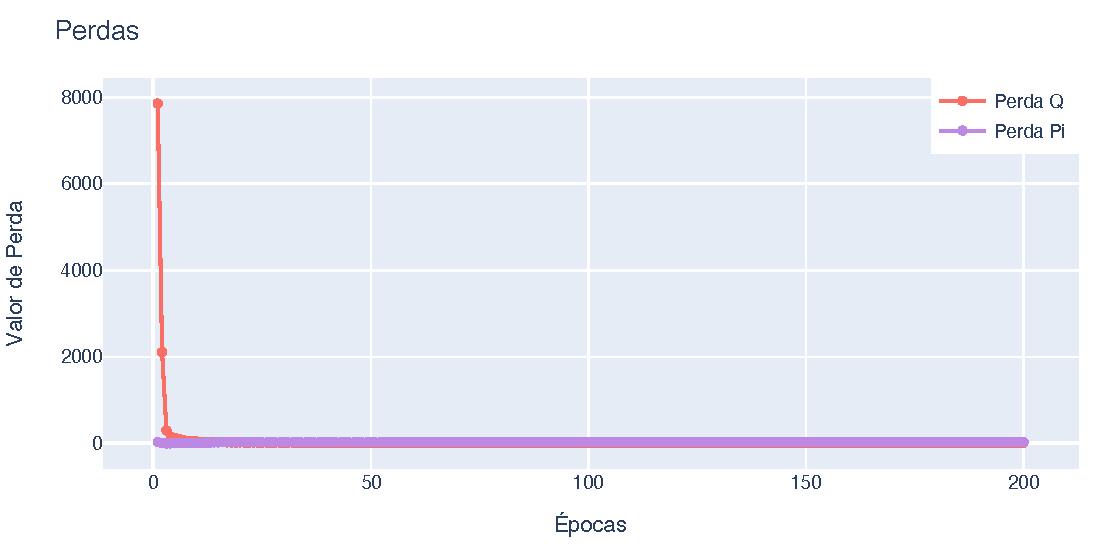
\includegraphics[width=\linewidth]{img/ddpg/abev3/clean/loss}
        \caption{ABEV3 - Comportamento das funções de perda.}
        \label{abev_clean_loss}
    \end{minipage}
\end{figure}

Nota-se na \refFig{abev_clean_ptrain}, que o lucro médio obtido durante a fase de treino, fica sempre perto de zero, mesmo apresentando dispersões de mil reais para mais ou para menos. Observa-se que a conversão para um valor de lucro constante não acontece de forma aparente, o que pode ser apenas o ruído presente nas ações, mas pode ser um indicio de que o algoritmo entrou em seu estado de \emph{deadlock}.

\figura[htbp]{img/ddpg/abev3/clean/profit_train}{ABEV3 - Lucro em treino}{abev_clean_ptrain}{width=.5\linewidth}

Quando o valor do lucro é analisado em teste (\refFig{abev_clean_profit}), percebe-se que a política de aversão a perdas, vista no ativo da VALE3 também foi aprendida. O agente termina a simulação com um nenhum lucro, mas também nenhuma perda, exatamente $0$, mesmo eventualmente o agente encontrando alguns lucros baixos de R\$$140,00$. Novamente, esse comportamento impede o aproveitamento do agente por lucros maiores, o que pode ser causado pela função de recompensa. Em relação as ações, apresentadas na \refFig{abev_clean_act}, o comportamento selecionado apresenta claramente o lucro de $0$, visto que o agente decide só vender desde o início da simulação, se avergindo a investir. Observe também que quando o agente tentou explorar as outras ações o agente obteve perdas significantemente maiores que ganhos, o que pode ter causado uma espécie de desistência pelo lado do agente. 

\begin{figure}[htbp]
    \centering 
    \begin{minipage}[b]{0.45\linewidth}
        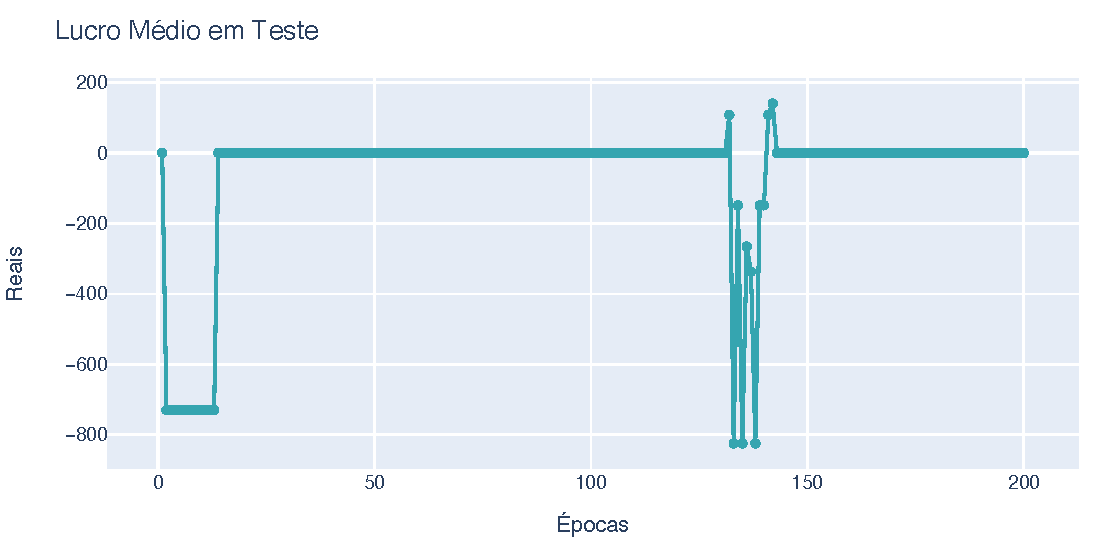
\includegraphics[width=\linewidth]{img/ddpg/abev3/clean/profit}
        \caption{ABEV3 - Lucro médio em teste.} 
        \label{abev_clean_profit}
    \end{minipage}
    \quad
    \begin{minipage}[b]{0.45\linewidth}
        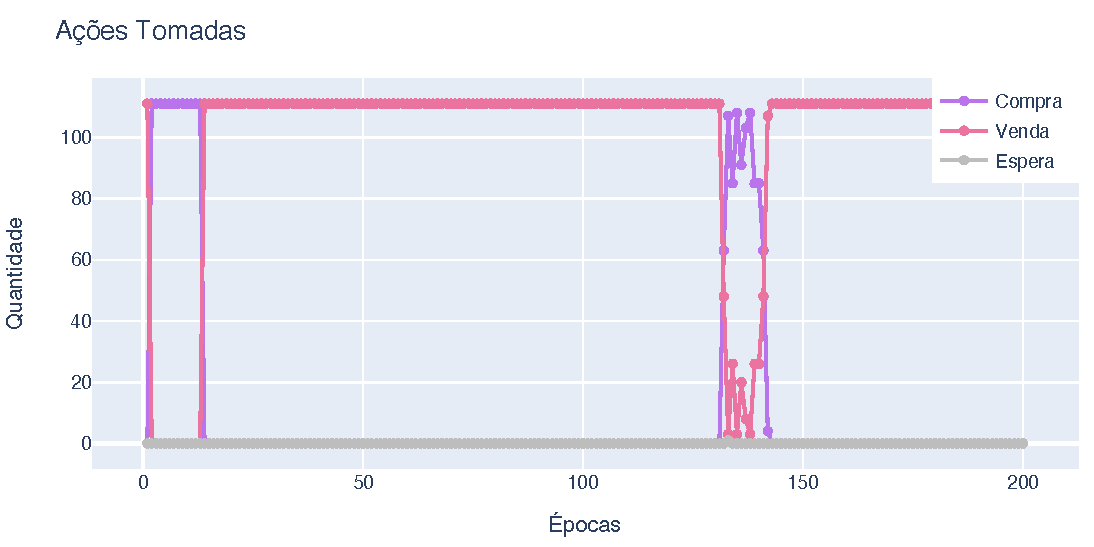
\includegraphics[width=\linewidth]{img/ddpg/abev3/clean/actions}
        \caption{ABEV3 - Quantidade de ações selecionadas em teste.}
        \label{abev_clean_act}
    \end{minipage}
\end{figure}

O desempenho do modelo para o ativo ABEV3 não é o esperado, no entanto, ainda assim o modelo evita a possibilidade de perdas. Este ativo, no início do período de investimento, estava sendo vendido a $17$ reais, mas no fim do período, o ativo chegaria a $15.54$, desvalorizando em $9,3\%$. Um investidor seguindo a estratégia \emph{buy and hold} possuiria grandes perdas nesse ativo. O que confirma mais uma vez, que a estratégia aprendida pelo agente, apesar de não ser ótima, consegue evitar prejuízos ao investidor.